% smth about how one of the most interesting features of KHM is the chiral Majorana edge modes. In general chiral edge modes are something that we look for in a variety of contexts. for example magnons and triplons - why are they useful?

As we saw in the previous chapter, the Kitaev model has turned out to be remarkably insensitive to changes in lattice geometry. Besides the TRS breaking effected by the presence of odd-sided plaquettes, we have shown that one can expect to find largely the same physics from a Kitaev model constructed on almost any trivalent lattice. If one were in the business of looking for new phases of matter, this result might be viewed as something of a disappointment! Such stability leave very little space for qualitatively new physics to be found simply by changing the board that the game is played on. 
Thankfully, nature is rarely so straightforward. The Kitaev model was originally proposed as a purely theoretical exercise \cite{kitaev_anyons_2006} -- with little expectation that any extant material could realise the bond-dependent spin couplings necessary for such a phase. However, following the initial proposal, it was suggested that one could engineer such couplings in certain transition metal compounds with strong spin-orbit coupling \cite{trebst_kitaev_2022,jackeli_mott_2009, chaloupka_kitaev-heisenberg_2010}. In the subsequent years, several material candidates were synthesised, such as the iridates Na$_2$IrO$_3$ and $\alpha$-Li$_2$IrO$_3$ \cite{singh_antiferromagnetic_2010, singh_relevance_2012,revelli_fingerprints_2020}, and later $\alpha$-RuCl$_3$ \cite{sandilands_scattering_2015,banerjee_proximate_2016}. In such `Kitaev materials', the Hamiltonian was shown to realise a dominant Kitaev-type bond-directional coupling, as well as other symmetry-allowed perturbations such as Heisenberg and $\Gamma$ couplings \cite{rau_generic_2014}. These perturbing interactions generally destroy the QSL phase, instead giving rise to a rich phase diagram with various long-range ordered magnetic phases~\cite{chaloupka_zigzag_2013,rau_spin-orbit_2016}. 

Remarkably, topological excitations persist even in these magnetically ordered phases. In the presence of a large magnetic field, the bulk magnon bands in these ordered phases can have nonzero topological invariants. Thus, they realise a magnonic equivalent of the quantum Hall effect, with surface states appearing with uni-directional propagation -- realising a so-called topological magnon insulator \cite{mcclarty_topological_2018,katsura_theory_2010,zhang_topological_2013,mook_edge_2014,mcclarty_topological_2022}. Hence, excitations of the (extended) Kitaev honeycomb model can be tuned from the chiral Majorana excitations (described in \textsection \ref{sec:chern_number_and_anyon_stats}) to stable chiral magnons as a function of increasing magnetic field. This is not only interesting theoretically but of direct experimental relevance -- both chiral magnetic excitations and chiral Majorana excitations give rise to a thermal Hall response~\cite{katsura_theory_2010,matsumoto_theoretical_2011}. The latter has been measured in the Kitaev magnet $\alpha$-RuCl$_3$~\cite{kasahara_majorana_2018,bruin_majorana_2022}, but whether its origin is related to QSL or TMI behaviour is still under debate~\cite{czajka_planar_2023,chern_sign_2021}.  

Unlike the QSL phase, the magnetically ordered phases that form in real Kitaev materials -- phases such as N\'eel, zigzag and stripy order -- are extremely sensitive to changes in the lattice geometry. For example, antiferromagnetic order depends on sublattice symmetry. By breaking this symmetry, one would expect to geometrically frustrate the formation of such phases, leaving space for more exotic ground states to form. In this chapter we will consider the star lattice, as a particularly simple example of a lattice that breaks sublattice symmetry. This lattice, shown in fig.~\ref{fig:star_lattice_and_jk}a, can be formed from the Honeycomb by decorating each vertex with a triangle. The Kitaev model on this lattice constituted the first rigorous example of a chiral QSL with {\it spontaneously} broken TRS, due to the presence of odd plaquettes \cite{yao_exact_2007} -- exactly the mechanism detailed in \textsection\ref{sec:fluxes_amorphous}. Despite much research on the stability of the Kitaev QSL on the honeycomb lattice~\cite{winter_models_2017,hermanns_physics_2018,trebst_kitaev_2022} the effect of perturbing interactions on the chiral Kitaev QSL has not been investigated on the star lattice. This is even more surprising given that the pure antiferromagnetic Heisenberg model on the star lattice is one of the rare established examples hosting a singlet VBS ground state phase with triplon excitations~\cite{richter_absence_2004,choy_classification_2009,yang_competing_2010, jahromi_spin-frac12_2018,jahromi_infinite_2018,ran_emergent_2018}. Additional motivation comes from the recent synthesis of the first $S=1/2$ materials realisation of the star lattice~\cite{sorolla_synthesis_2020,ji_dielectric_2022} (previous star lattice realisations contained $S=5/2$ spin clusters~\cite{zheng_star_2007}).  

In this chapter we will investigate the rich ground state phase diagram and distinct types of chiral excitations of the Kitaev-Heisenberg model on the star lattice. Here, the presence of odd plaquettes (and thus the frustration of N\'eel order) leads to the formation of a valence bond solid (VBS). In its most common form, a VBS is created by neighbouring pairs of spins anti-aligning into singlets, forming a dimer covering of the entire lattice -- however, we also find a more exotic `triplet VBS', where neighbouring bonds couple into bond anisotropic triplet states. On a singlet VBS background, excitations involve breaking a singlet and creating a spin-1 triplet -- a so-called triplon mode that can be represented as a bosonic particle~\cite{sachdev_bond-operator_1990}. Recently, interest has been generated in triplons as a way of realising a bosonic bulk-boundary correspondence. This has been proposed both in 1D topological chain systems~\cite{joshi_topological_2017}, as well as 2D bosonic analogues of the quantum Hall effect~\cite{romhanyi_effect_2011,romhanyi_hall_2015,mcclarty_topological_2017, nawa_triplon_2019, malki_magnetic_2017}. In general, such effects have relied on the presence of Dzyaloshinskii-Moriya (DM) interactions to generate complex hoppings in the triplon Hamiltonian, allowing for non-zero Chern and winding numbers to appear. Here, we will show that the Kitaev interaction provides an alternative route for a triplon Hall state forming in the absence of DM interactions and unearth an extremely rich phase diagram with a wide range of Chern numbers. Thus, we establish that -- in analogy to the honeycomb Kitaev model, which can be tuned with a magnetic field from hosting chiral Majorana to chiral magnon excitations -- the Kitaev-Heisenberg model on the star lattice tunes from chiral Majoranas to chiral triplons. 

\begin{figure}[t]
    \centering
    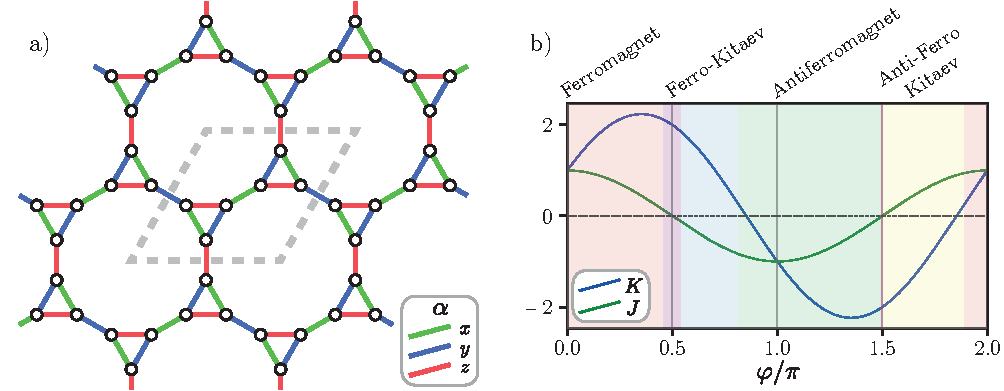
\includegraphics[]{kitaev_heisenberg_star/figures/star_lattice.pdf}
    \caption{ 
        \textbf{(a)} A fragment of the star lattice is shown. Bond labelling is indicated by the colouring, and the six-site unit cell is depicted with a grey dashed rhombus.
        \textbf{(b)} The dependence of the $J$ and $K$ values on the parameter $\varphi$ is shown. The two pure Heisenberg and two pure Kitaev points are labelled. The background colouring corresponds to the phase boundaries obtained in \textsection\ref{sec:triplons_dmrg}.
    }
    \label{fig:star_lattice_and_jk}
\end{figure}

The structure of this chapter is as follows. 
First we introduce the model, describing the parameters used to tune the system and discussing previous studies that have looked at both the star and the honeycomb lattices. Following this, our investigation is composed of three parts. 
In \textsection\ref{sec:triplons_dmrg} we start by numerically characterising the ground state phase diagram using infinite density matrix renormalisation group (iDMRG) methods. In particular, we find two phases in the star lattice that do not have an analogue on the Honeycomb lattice, where geometric frustration leads to the formation of a VBS ground state. We will also present a \textit{four-unit-cell spin rotation} that reveals a hidden isometry of the ground state phase diagram. We show that the four non-spin liquid phases may be categorised into two sets, which are equivalent under this transformation.
In \textsection\ref{sec:majorana_mft} we construct a parton Majorana mean field description that corroborates the ground state phase diagram, and allows us to determine the topological properties of the bands and the presence of chiral Majorana excitations in the extended KSL regime. 
Finally, in \textsection\ref{sec:triplon_bond_operator} we  construct a bosonic mean field theory describing the triplon excitations of the VBS phase. The topological properties of the triplon phases are derived and we confirm the existence of topologically protected triplon edge modes. 

Let us start by defining the model, which we shall construct on the star lattice shown in fig.~\ref{fig:star_lattice_and_jk}a. As in the previous chapter, each site hosts a single spin-1/2, and bonds are coloured with a label $\alpha \in \{x,y,z\}$ such that no vertex touches two bonds of the same colour. We choose the Hamiltonian to interpolate between two well-studied limits: the spin isotropic Heisenberg and the anisotropic Kitaev limit. In the Heisenberg limit, adjacent spins are coupled with an isotropic $\mathbf{\sigma}_j \cdot \mathbf{\sigma}_k$ coupling. In the Kitaev limit each bond of type $\alpha$ is coupled by a $\sigma_j^\alpha \sigma_k^\alpha$, thus only in the direction that matches the colouring.
\begin{align} \label{eqn:kitave_heisenberg_hamiltonian}
    H = -
    \sum_{\braket{jk}_\alpha } \bigg (K \sigma_j^\alpha \sigma_k^\alpha
    +J \sum_{\bar \alpha \neq \alpha}  \sigma_j^{\bar \alpha} \sigma_k^{\bar \alpha}
    \bigg ).
\end{align}
Here $\braket{jk}_\alpha$ indicates a bond of type $\alpha$ that connects adjacent sites $j$ and $k$. The parameter $K$ determines the strength of the ``on-colouring'' coupling, where the coupling direction matches $\alpha$, and $J$ determines the strength of the two remaining ``off-colouring'' couplings. In analogy with previous studies~\cite{chaloupka_zigzag_2013, gohlke_dynamics_2017}, let us introduce a single parameter $\varphi \in [0,2\pi]$ that smoothly maps onto the possibilities for $K$ and $J$ according to
\begin{align} \begin{aligned} \label{eqn:phi_def}
    K &= 2\sin \varphi + \cos \varphi, \\
    J &= \cos \varphi,
\end{aligned}\end{align}
shown in fig.~\ref{fig:star_lattice_and_jk}b. 